\documentclass{article}
\usepackage[utf8]{inputenc}
\usepackage{times}
\usepackage{bm}
\usepackage{etoolbox}
\usepackage[english]{babel}
\usepackage{biblatex}
\usepackage{amsmath}
\usepackage{amsfonts}
\usepackage{listings}
\usepackage{algorithm}
\usepackage{graphicx}
\usepackage{caption}
\usepackage{subcaption}
\usepackage[noend]{algpseudocode}
\usepackage{verbatim}
\addbibresource{references.bib}
\usepackage{hyperref}
\usepackage{float}
\usepackage{csquotes}
\usepackage[table,xcdraw]{xcolor}
\def\infinity{\rotatebox{90}{8}}
	\definecolor{trolleygrey}{rgb}{0.5, 0.5, 0.6}
\hypersetup{
    pdfpagemode={UseOutlines},
    bookmarksopen,
    pdfstartview={FitH},
    colorlinks,
    linkcolor={blue},
    citecolor={red},
    urlcolor={blue}
  }

\renewcommand{\algorithmiccomment}[1]{\textit{#1}}

\title{Operational Research Project Report\\ \textbf{Robust Knapsack Problem}}
\author{Group 1\\A. Baldo, V. Baldoni, M. Boffa, L. Cascioli, C. Lanza, A. Ravera}
\date{July 2020}

\begin{document}

%\maketitle

\section{Introduction to the problem}
The Robust Knapsack Problem (RKP) is an NP-hard problem based on an extension of the well-known Knapsack Problem (KP). As for the KP,  the RKP  is based on a set of items \textit{N = \{1,...,n\}}, each one characterized by its own positive profit $p_i$ and a certain weight $c_i$; items can  fill the knapsack up to its capacity \textit{W}. The RKP behavior detaches from the KP by introducing variability in the data, and especially in the weights and profits deriving from the chosen items. In particular, items can have three possible costs \textit{\{$c_i^l$, $c_i^a$, $c_i^u$\}}, with \textit{$c_i^l$ $\leq$ $c_i^a$ $\leq$ $c_i^u$},  and at most $\Gamma$ items can change their weight from the nominal value $c_i^a$. Furthermore, the presence of both items \textit{i} and \textit{j} can lead to an additional contribution in the overall profit computation, either positive or negative, which will be called \emph{synergy}. Of course, several different  interpretations can be thought to approach this problem; the one  given in this paper sees the knapsack as the available budget of a set company. Items are investments in which the company is interested in, and the uncertainty related to their costs is due to credit lines that the company will be able to open; eventually, the opening of two investments \textit{i} and \textit{j} may generate synergies that can lead to an extra profit. The objective is to maximize the minimum possible profit taking into account the uncertainties, obviously respecting the budget limits.

\section{Review of the literature}
The RKP problem has attracted some interest in recent years and has been addressed by several researchers and academics; some of these results and proposals were analyzed and taken into account for the development of this work. \\

In the definition of the LP model, references from previous works were exploited. Namely, the paper from \textit{Bertsimas and Sim} \cite{price} provides a detailed historical overview on how different solutions were thought and refined with time, not only for the RKP problem but for treating robustness in general. Then, the paper from \textit{Monaci et al.} \cite{Monaci} was very useful for this specific work. It brought both additional clarity on the model and, citing also the work of Klopfenstein and Nace \cite{Klopfenstein}, it presents an exact dynamic programming algorithm for the RKP without, though, introducing the concept of the \emph{synergies}. This was in any case very useful to understand and first experiment a first alternative solution method to the linear model. Moreover, the paper also provided the idea of adopting a graph for the modelling of the problem, which was the basis, in the end, for one of the developed heuristics. 

\section{Instance generation}
The creation of several well differentiated instances of the problem represented a first notable task, especially when it was time to look for the limits and problems of the heuristics that were being implemented. An ad-hoc script was created to generate them, trying to determine a good trade-off between differentiation among the datasets and settings created on purpose in order to put the heuristics in the trickiest conditions. 

A first generation round created uniformly distributed investments, with coherent values of costs, profits and synergies. To add a bit of complexity, the synergies terms were also thought to assume negative values. The main differentiation involved the variation of the core variables characterizing the instance, i.e. the number of items, the maximum number of deviating items $\Gamma$, and the knapsack capacity/size. \\
Subsequently, some particular instances (e.g. where no investments at nominal cost were to be included in the optimal solution) have been built to test the methods in unusual conditions, but no particular problems were discovered. \\
A final third round of instances generation tried to differentiate the distribution of the data (e.g. using Gaussian distributed data) and it included some examples of profits smaller than the corresponding "uppered" costs, in order to identify new situations where the algorithms could be tested.\\

%%%dataset naming
For what concerns the nomenclature of the \emph{config files}, instances with less than 45 items were called \emph{small}, bigger instances up to 100 items were said to be \emph{medium}, and the largest one were named \emph{big}, following this class with the values of $n_{items}$, $\Gamma$ and the capacity.

\section{Mathematical model}
Having clear in mind the statement of the problem and some of the previous works that addressed similar tasks, the first thing to do was the development of a MILP model for the exact description and solution of the problem. \\

The constants and variables used in its definition are here briefly described.

\subsubsection*{Constants}
\begin{itemize}
    \item W: capacity of the knapsack;
    \item N: total number of investments at disposal;
    \item $\Gamma$: maximum number of items whose cost can change from the nominal value;
    \item $p_i$: profit associated to the activation of investment \emph{i}
    \item $s_{ij}$: additional synergy if investments \emph{i} and \emph{j} are activated;
    \item $c_i^a$: nominal cost of investment \emph{i};
    \item $c_i^l$: lower cost of investment \emph{i};
    \item $c_i^u$: upper cost of investment \emph{i}.
\end{itemize}
\subsubsection*{Variables}
\begin{itemize}
\item $x_i \in \{0,1\}$\space$\forall i$: it tells whether the investment \emph{i} is active (=1) or not (=0);
\item $y_{ij} \in  \{0,1\}$\space$\forall i,j$: it tells whether the synergy between investments \emph{i} and \emph{j} must be activated. Hence, it is equal to 1 only if both the items are inserted into the knapsack.
%\item $\rho \geq 0$, $\pi_{i} \geq 0$\space$\forall i$: dual variables for the costs treatment. 

\end{itemize}

\subsubsection*{Model}

A first formulation of the model has as objective function (i.e. total earning to be maximized) an expression like the following: \[ max \sum_i p_i * x_i + \sum_{ij} s_{ij} * y_{ij} - (max_{c_i} \sum_i c_i*x_i).\] The last term, related to the costs, expresses the concept of \textit{worst-case} scenario with a sub-problem of maximization of the costs for the chosen set of investments. Such term, therefore, is also present in the capacity constraint which is of the form: \[max_{c_i} \sum_i c_i*x_i\leq W\] where $c_i$ is the general cost assumed by the investment \textit{i}.\\
For the modeling of the synergies, the variables $y_{ij}$ and $x_i$ have been linked with the following constraints:
\begin{itemize}
        \item $y_{ij} \geq x_i+x_j-1$
        \item $y_{ij} \leq x_i$
        \item $y_{ij} \leq x_j$ \space\space\space\space\space$\forall i,j$.
    \end{itemize}
    
These constraints express the conditions under which a synergy is considered: when both the investments are activated, the additive profitable term is activated too, being this substantially a simple logical AND statement. \\

%duality
The two sub-problems of maximization related to the costs can be treated with the aid of \textit{duality}, in order to transform them into minimization problems which are easier to be linearized. 
The capacity constraint, modifying the term $max_{c_i} \sum_i c_i*x_i$ (present also in the objective function), can be decomposed as:
\[ \sum_i c_i^a * x_i + max \sum_i \hat{c_i} * x_i \leq W\] 
where the $\hat{c_i} \in [0, c_i^u-c_i^a]$ represent the deviations from the nominal costs introduced in the worst-case scenario. It must be taken into account that a bound must be set on these $\hat{c_i}*x_i$: at most $\Gamma$ items can assume their upper cost.
The focus for the maximization is in practice shifted towards the last part of the expression, which, from what has been said, can be modelled as following:
\[ max \quad \sum_i [\hat{c_i}*x_i]*z_i \]
\[\sum_i z_i \leq \Gamma\]
\[ z_i \leq 1 \quad \forall i\]
\[ z_i \geq 0 \quad \forall i.\]
This brings to a new linear sub-problem where the $\hat{c_i}$ and the $x_i$ are the coefficients for the introduced variables $z_i$, which must be continuous in order to apply the \emph{duality} transformation. Practically, once an assignment has been done for the $x_i$, this sub-problem `chooses' the worst possible $z_i$ to be set to 1 (at most $\Gamma$), taking at upper cost those items that maximize the total cost for the chosen set of investments. In order to apply duality, a matricial formulation may be of great help. The canonical matrices and vectors can be defined as follows, being $c \in \mathbf{R^{N,1}}$, $A \in \mathbf{R^{N+1,N}}$ and $b \in \mathbf{R^{N+1,1}}$: 

\[ c=
        \begin{bmatrix}
            \hat{c_1}*x_1\\
            \dots\\
            \hat{c_i}*x_i\\
            \dots
        \end{bmatrix}, 
    ~A =
        \begin{bmatrix}
        1 & 1 & ... & 1 & 1\\
        &&&&\\
        &&\begin{pmatrix}
        &&I&&
        \end{pmatrix}&&\\
        %&&I&&\\
        &&&&
        \end{bmatrix},
    \\~b=
        \begin{bmatrix}
        \Gamma\\
        1\\
        \dots\\
        1
        \end{bmatrix}.
\]

Having done so, the problem can be re-expressed in the `standard' form as shown below on the left, being $z \in \mathbf{R^{N,1}}$ a column vector with all the $z_i$ variables. From that, the equivalent dual problem is obtained as follows using the theory of \emph{duality}:

\[
\begin{array}{lll}
max \quad c^T*z\\
s.t. \quad A*z \leq b\\
\quad \quad ~~ z \geq 0
\end{array}
\Leftrightarrow
\begin{array}{lll}
min \quad b^T*\lambda\\
s.t. \quad A^T*\lambda \geq c\\
\quad \quad ~~ \lambda \geq 0 
\end{array}
\]

Having already defined \emph{A}, \emph{b} and \emph{c}, all the needed elements except  $\lambda$ have been presented. For what concerns the new dual variables, it has been chosen, in order to keep a notation equivalent to that used in the reference paper \cite{Monaci}, to build the vector $\lambda \in \mathbf{R^{N+1,1}}$ of the Lagrangian multipliers as:
\[
\lambda =
\begin{bmatrix}
        \rho\\
        \pi_1\\
        \dots\\
        \pi_i\\
        \dots
        \end{bmatrix}.
\]



At this point, substituting the introduced vectors and matrices in the general dual problem, the formulation becomes:
\[ min \quad \Gamma*\rho + \sum_i \pi_i \] \[ \rho + \pi_i \geq \hat{c_i} * x_i \quad \forall i\]\[ \rho \geq 0, \pi_i \geq 0 \quad \forall i.\]
%The new dual variables $\rho$ and $\pi_i$ are simply the Lagrangian multipliers for the constraints on the $z_i$.\\
Therefore, the initial capacity constraint can be reformulated (with the addition of the new constraints for the dual variables) as: 
\[ \sum_i c_i^a*x_i + min~(\Gamma * \rho + \sum_i \pi_i) \leq W.\] The \emph{min} is actually no more necessary, as the nature of the main problem, which aims at maximizing the value of the objective function (the profit), will necessarily bring the expression of the costs to its minimum possible value. Deleting the \emph{min}, the feasible space is expanded, but the final result will be the same.\\

An equivalent reasoning can be performed for the term $max_{c_i} \sum_i c_i*x_i$ in the objective function, and it has been verified that the same $\rho$ and $\pi_i$ variables may be uniquely adopted for both the cases, so that in practice each of the secondary maximization problems $max_{c_i} \sum_i c_i*x_i$ can be simply substituted with:
        \[
        \sum_i c_i^a * x_i + (\Gamma * \rho + \sum_i \pi_i) \]
        introducing in the model the dual constraints: 
        \[ \rho + \pi_i \geq \hat{c_i} * x_i \quad \forall i\]
        \[\rho \geq 0,~\pi_i \geq 0 \quad \forall i. \]

The final formulation of the model for the RKP problem is therefore the following.\\
\\
\emph{max z}
\\s.t.
\begin{itemize}
    \item earning in the worst case to be maximized:\\ $z \leq \sum_i p_i*x_i + \sum_{i,j} s_{ij}*y_{ij} - \sum_i c_i^a*x_i - (\Gamma*\rho + \sum_i \pi_i)$;
    \item knapsack capacity constraint:\\$\sum_i c_i^a*x_i + \Gamma*\rho + \sum_i \pi_i \leq W$;
    \item duality constraints:\\ $\rho + \pi_i \geq (c_i^u - c_i^a)*x_i $ \space\space\space$\forall i$;
    \item synergies activation constraints:
    \begin{itemize}
        \item $y_{ij} \geq x_i+x_j-1$
        \item $y_{ij} \leq x_i$
        \item $y_{ij} \leq x_j$ \space\space\space\space\space$\forall i,j$.
    \end{itemize}
   \item variables domains:\\$ x_i \in \{0,1\} ~~\forall i, \quad y_{ij} \in \{0,1\} ~~\forall i,j, \quad \rho \geq 0, \quad \pi_i \geq 0 ~~\forall i$.
\end{itemize}

\section{Model results}
By performing some quick trials on small instances whose correct solution could be checked by hand, it was possible to assert the correct functioning of the developed model (run on the \textit{pulp} solver). Therefore, some specific instances of the problem were subsequently prepared in order to analyze the evolution of the behavior of the model varying some specific input parameters, both in terms of the solution itself and in terms of execution time.\\

\begin{figure}[!ht]
\centering
{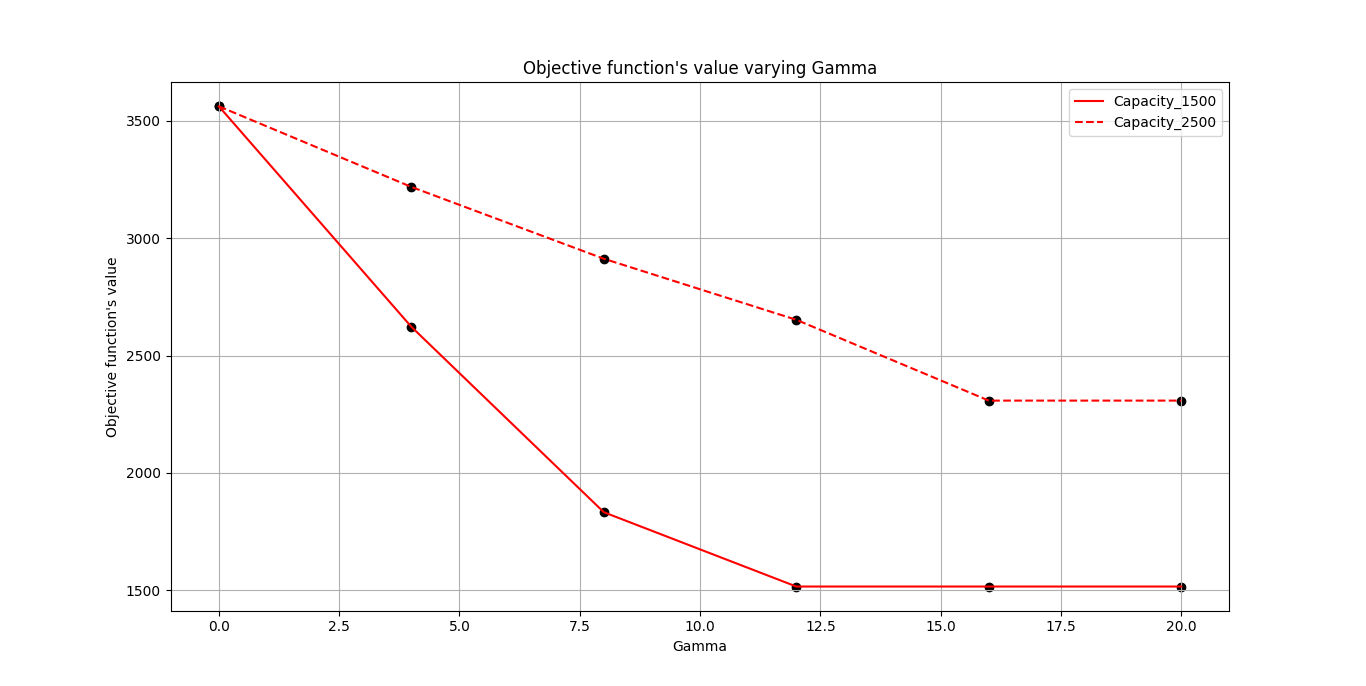
\includegraphics[width=0.75\textwidth]{Objective_function_model_2.png}}
\caption{Variation of the solution for increasing $\Gamma$ and two different capacities}
\label{model_1}
\end{figure}

Fig.~\ref{model_1} shows some first rather expected results. Both the lines are related to a general problem with fixed number of investments and same profits, synergies and costs. The continuous line represents a scenario where the capacity has been fixed to a value (1500), while the dashed line has a bigger capacity, equal to 2500 (hence its solution will contain more items, so it will be higher).  \\

As mentioned, when $\Gamma=0$ the scenario is that of a classic KP problem, where all the cases share the same basis and therefore reach the same result. Going along the x axis, $\Gamma$ increases, meaning that more and more investments will be forced to assume their upper cost. This inevitably makes the final solution gradually decrease, as the costs will for sure increase, and at some point it may be even possible that the items in the previous solution cannot be all fitted into a solution where $\Gamma$ is bigger. This is the so called \textit{price of robustness}: it must be taken into account that the least favourable combination of costs will be realized, and countermeasures must be taken to maximize the earning in such situation. Since the introduced cost variations are remarkable, the optimal solution heavily decreases, until at some point it reaches a constant `boundary' value: it means that less than $\Gamma$ elements are fitted into the solution, thus a further increase of $\Gamma$ cannot influence the result anymore. Clearly, having fixed profits and costs, the smaller the knapsack size, the sooner this will happen. \\
Of course, each basic setting behaves differently from the others due to its peculiar numerical characteristics, but the general trend for the impact of $\Gamma$ on the solution is that expressed in the previous figure. \\

For what concerns the execution times, it was easily noticed how, increasing the number of investments in the instance of the problem, the model starts to struggle pretty quickly; indeed, when more than 40-45 items are present, the solver takes several minutes (if not hours) to find the optimal solution, and it is almost impossible to run it on even bigger instances. This will be also shown later in fig.~\ref{times}.\\


No particular dependence has been noted, despite some ideas and experiments that were made, between the execution time and the capacity or the ratio between $\Gamma$ and $n_{items}$.
That said, in order to get solutions in cases much larger than those solvable by the model, heuristic methods needed to be defined.

\section{Heuristics}
Once the model had been correctly implemented and tested, it was time to work on the definition of some heuristic methods in order to find a good solution sufficiently close to the optimum within a time much more affordable with respect to the model. The first attempt followed the dynamic programming approach presented by \textit{Monaci et al.} \cite{Monaci} for the RKP problem without synergies. After having implemented the model shown in the paper, though, the requirement of improving the method with the addition of the synergies proved to be practically impossible, at least for the different ideas that were tested; in such dynamic programming approach, indeed, the real-time evaluation of all the possible combinations of profits, costs and synergies cancelled out the advantages of ordering the investments for a progressive and guided filling of the knapsack. 
After some struggling, therefore, another path was chosen to build an heuristic, and also in this case the idea came from the same reference paper.
\subsection{Graph Heuristic}
The first and main functioning heuristic that was developed is named `Graph Heuristic'. It was born, as mentioned, after some hints illustrated by the paper of  \textit{Monaci et al.} \cite{Monaci}, according to which a graph representation of the problem could be used to define an optimal `path of investments'. The main idea is to build a fully-connected directed graph, where each node (i.e. each investment) can reach any other node with a directed arc. Actually, arcs are coupled and from a node to another a \textbf{heavy arc} and a \textbf{light arc} exist: the first means that the destination node is being added to the solution with its upper cost, the second that it is taken with its nominal cost.
Of course, the last event is possible only if $\Gamma$ items have already been inserted. A pseudo-code that explains the general structure of the algorithm is presented below in algorithm~\ref{pseudo_code_graph}. \\

The algorithm basically creates at each iteration a different sub-optimal feasible path, starting each time from a different node and proceeding `greedily', selecting at each step the most convenient arc to pick. This is done, as sketched in the pseudo-code, by sorting both the heavy and the light arcs taking as \textit{score} the profit brought by the destination node minus its cost (upper when heavy arc, nominal when light arc), and then summing the contributions of the synergies arising with the insertion of the node in the current solution. Many other methods for the sorting of the arcs have been tested, but this resulted by far to be the most efficient one, as it perfectly reflects the intent of the objective function, which is the maximization of the total income given by the current solution. \\

%sketch pseudocode
\begin{algorithm}[H]
\caption{Graph Heuristic}\label{graph}
\begin{algorithmic}[1]
\State \textsl{bestSol}=0, \textsl{bestPath}=[]
\For {\textsl{n} in nodes}
    \State initialize new solution starting from node \textsl{n}
    \While {items can be added to the solution}
        \State sort arcs from last node to all the nodes not in \textsl{current solution}
        \State {\color{trolleygrey}{\#heavy arcs: profit + synergies - costUpper}}
        \State {\color{trolleygrey}{\#light arcs: profit + synergies - costNominal}}
        \If {len(\textsl{current solution})$ < \Gamma$}
            \State insert into \textsl{solution} the first feasible heavy arc (if any)
            \State evaluate \textsl{current solution}
            \If {\textsl{current solution} is better than \textsl{bestSol}}
                \State update \textsl{bestSol} and \textsl{bestPath} with \textsl{current solution}
            \EndIf
        \Else
            \For {\textsl{arc} in light arcs}
                \State pick \textsl{arc} as best available light arc 
                \State check hypothetical new solution with \textbf{Build\_Destroy}
                \If{feasible}
                    \State insert \textsl{arc} into \textsl{current solution}
                    \If {\textsl{current solution} is better than \textsl{bestSol}}
                        \State update \textsl{bestSol} and \textsl{bestPath} with \textsl{current solution}
                    \EndIf
                    \State exit
                \Else
                    \State remove \textsl{arc} from \textsl{current solution}
                    \State {\color{trolleygrey}{\#try again with the next light arc}}
                \EndIf
            \EndFor
        \EndIf
    \EndWhile
\EndFor\\
\Return {\textsl{bestSol},\textsl{bestPath}}

\end{algorithmic}
\label{pseudo_code_graph}
\end{algorithm}

After the sorting, the choice of the node to add is determined by the heavy/light arc which guarantees the best improvement, as well as the respect of the constraints in terms of capacity. Indeed, if an investment with upper cost is taken (i.e. if less than $\Gamma$ items are inside the current solution), the first heavy arc which fits into the remaining capacity is taken. Instead, when $\Gamma$ or more items are already present, the algorithm tries to insert a node through a light arc; this, however, is not an immediate task. Looking at the problem using an \textit{adversarial game} interpretation, it can be assumed in this case that an adversary has the ability to bring at most $\Gamma$ investments to upper cost, and he does so as to penalize as much as possible the current solution. In fact, the goal of the problem is to maximize the profit for the worst-case scenario, so that where the total highest possible cost for the chosen investments is realized. Therefore, when an item is added through a light arc, it is not automatic that such item will be effectively taken at nominal cost: the adversary could upper it and lower another one if this creates in the end an higher total cost, which could even exceed the knapsack capacity. Subsequently, an ad-hoc function called \textbf{Build-Destroy} has been implemented to deal with this issue. Each time that a light arc is taken, the resulting solution (with the destination node taken at nominal cost) is passed to the function; the output will be a solution equal to the input if the adversary has no gain in upgrading the cost of the new item in spite of that of another one previously taken at upper cost; but if, instead, the insertion allows the adversary to further worsen the total cost with such actions, the function understands it and acts to provide some countermeasures. Indeed, it sorts the items in the solution so that it has the highest possible value for the cost (hence taking with upper cost the worst possible items), and it takes away from the solution the least beneficial elements until it becomes feasible again. So when a light arc is taken, if in the end the item is truly added (after passing through \textbf{Build-Destroy}) the solution is really updated, otherwise the last step is deleted because it was not actually acceptable, and the next light arc is considered. \\

This procedure goes on until no more space is available for a new item in the knapsack. At that point, the current solution is flushed and a new path is established from a new starting node. Each time that an update is made to the current solution, of course, a comparison is made with the best solution found up to that moment: if the current state is bringing an improvement, the value of the solution and the path in the graph leading to it are updated, so that in the end the best value (which is hopefully the optimum) will be displayed.

\subsection{Genetic Heuristic}
An alternative heuristic method was developed around the theoretical idea of the \emph{genetic algorithms}. The basic structure is composed of four main steps; a pseudo-code showing the structure of the procedure is presented below in algorithm~\ref{model_gen}.

\subsubsection{Creation of the population}
This is a sort of initialization of the algorithm. It should provide a sufficiently diversified basis needed by the following, core part of the procedure, where improvements are made in order to reach the optimum starting from an already good point.\\

Therefore, the creation of the population follows a procedure which aims at finding a reasonable trade-off between a fast initialization and an acceptably good, rough estimation of a sub-optimal solution. The procedure consists in creating $n_{items}$ different solutions, each one initialized starting with a different item. Then at each step the investment whose deviation $upper\_cost-nominal\_cost$ is the highest (among those not already inserted) is added to the solution. In this way an initial solution is built, constantly checking the feasibility of the partial solution that is being developed. The first $\Gamma$ elements are chosen with their upper costs, while the remaining ones (when present) are considered with nominal cost. This sorting method for the initialization showed good performances for most of the datasets; sometimes, though, it erroneously stucks the solution around some local maxima. A specific \textbf{re-initialization} function was hence implemented to deal with these cases. It is applied when the core part of the algorithm does not get any improvement after a given number of iterations, and its aim is to apply a different initialization paradigm in order to explore different solutions. The creation of the new population simply changes the criterion according to which an item is added to the solution, following an approach equivalent to that used in `Graph Heuristic': the chosen node $x$ now maximizes the metric:
\begin{equation*}
    profit_x-upper\_cost_x+synergies_{x,y}\quad \forall y\in current\_solution.
\end{equation*}
This method has already showed good results in the case of `Graph Heuristic' and, indeed, it seems to be of help in the cases which performed poorly with the previous mathematical rule.

\subsubsection{Main Procedure}
Once the rough basis has been evaluated, the main procedure, using some concepts belonging to the family of the \textit{genetic algorithms}, acts on the population of solutions in order to refine them and bring them closer to the optimum. 
\paragraph{Parents selection}
This procedure basically selects the best `parents' to be combined together, in order to produce new solutions that should represent, at each iteration, an improvement towards the optimal solution. The evaluation of a so called \textbf{fitness score} defines if a \emph{parent} solution is likely to generate useful \emph{sons}. Its definition logically followed the idea behind the objective function of the problem, evaluating for each solution the sum of the total profits and synergies, subtracting the term related to the total costs of the investments. \\

Since the general mechanism of a genetic algorithm causes a rapid expansion of the population, then, each time only the best $n_{items}$ \emph{parents} are kept, to act on the most meaningful elements and avoid an explosion of the population size, keeping a  proportionality with the size of the dataset. 
\paragraph{Crossover}
This is the core of any genetic algorithm; it determines how the parents should be `coupled' for the evolution of the population. The general pattern requires to define a crossover point in the pair of \textbf{chromosomes} (i.e. the parents), where a break is performed to then merge two halves coming from different parents, generating two new elements from each pair of chromosomes. The crossover point is each time randomly chosen. \\

After having noticed that the crossover operation has a big impact in the first iterations, but it is not efficient to obtain a refinement of an already good solution, the parents involved in the crossover procedure were slightly decreased at each iteration, to speed up the process. Instead, the last improvements are possible thanks to the next step, the \emph{mutation}.
\paragraph{Mutation}
It is the final but essential passage, as it introduces unpredictability in the evolution of the solutions without heavily upsetting the outputs of the crossover. A mutation generally looks for another item, not belonging to the current solution, which could bring the maximum possible improvement in terms of objective function maximization. This item takes the place of another random element in the solution. Instead, if all the possible elements are already included in the current solution, the mutation simply deletes a random element without inserting anything. Clearly, this kind of operation, thought to bring an improvement, could as well make the solution infeasible. Therefore, after the mutation, the feasibility of the new solution is checked: in case the new solution is infeasible, the last element is deleted, and this is repeated until the feasibility is met again. \\

These three steps are repeatedly performed until a sort of convergence criterion is met; more specifically, by checking the behaviour of the optimal solution in the current population through the last five iterations. This guarantees a bound for the execution time and allows to identify whether the algorithm resulted stuck in local maxima, which represent the main threat for this algorithm to succeed.


\begin{algorithm}[H]
\caption{Genetic Heuristic} \label{genetic}
\begin{algorithmic}[1]
\State \textsl{bestSol} = [0,0], \hspace{0.5cm} \textsl{population} = [], \hspace{0.5cm} \textsl{reinitialization} = False
\State \textsl{sortingFunction} = upperCost - nominalCost
\State \textsl{fitnessScore} = profits - costs + synergies
%\State \textbf{• Create Population} \#\textit{threads}
\State {\color{trolleygrey}{\#create population}}
\For{\textsl{item} in items}
    \State create an initial \textsl{Solution} starting from \textsl{item}
    \While{ len(\textsl{Solution}) != $\Gamma$}
        \State sort remaining items according to $sortingFunction$ 
        \State add first item at uppered cost to \textsl{Solution}
        \If{\textsl{Solution} not Feasible}
            \State remove item
        \EndIf
    \EndWhile
    \State sort remaining items according to $sortingFunction$
    \For{\textsl{i} in remaining items}
        \State add \textsl{i} at nominal cost to \textsl{Solution}
        \If{\textsl{Solution} not feasible}
            \State remove item
        \EndIf
    \EndFor
     \State add \textsl{Solution} to population
\EndFor

 

%\State \textbf{• Main Procedure}
\State {\color{trolleygrey}{\#main procedure}}
\For{\textsl{i} in range(len(items))}
    \State {\color{trolleygrey}{\#parents selection}}
   %\State \textbf{• Parents' Selection}
    \State  remove duplicates from population
    \State  sort population according to decreasing \textbf{fitnessScore}
    \State  $parents$ = first $len(item)$ solutions of the population
    \State  $reducedParents$ = subset of size inversely proportional to $i$
    \State  create $reducedParents\times(reducedParents-1)/2$  couples
    
    \algstore{myalg}
    \end{algorithmic}
    \label{model_gen}
    \end{algorithm}
    \begin{algorithm} [h!]                    
    \begin{algorithmic} [1]
    \algrestore{myalg}
    
   %\State \textbf{• Crossover} \#\textit{threads}
   \State {\color{trolleygrey}{\#crossover}}
    \For{\textsl{couple} in couples}
        \State determine random crossover point
        \State create two siblings by merging the opposite halves of the two parents
    \EndFor
    

    
    %\State \textbf{• Mutation} \#\textit{threads}
    \State {\color{trolleygrey}{\#mutation}}
    \State  $ probability$ = min(0.2*(1+i), 1)
    \For{\textsl{sibling} in siblings}
        \State $rN$ = random number
        \If{$rN < probability$}
            \State $rP$ = random position to mutate
            \State \{\textsl{missing items}\} = \{total items\} - \{items in the solution\}
             \If {any \textsl{missing item}}
                \State sort \textsl{missing items} with $profits-costs+synergies$ decreasing
                \State swap best \textsl{missing item} with the item at $rP$
            \Else
                \State remove element at $rP$
            \EndIf
            \While{\textsl{solution} not feasible}
                 \begin{comment}
                \State sort \textsl{solution} with $sortingFunction$ 
                \end{comment} 
                \State remove last item
            \EndWhile
            \State add \textsl{sibling} to population
        \EndIf
    \EndFor
       
       
    
    %\State \textbf{• Get optimum} from current population
    \State {\color{trolleygrey}{\#find optimum for the current population}}
    \State update $bestSol$ with solution and fitnessScore
   
    \If{\textsl{i}$>$5 \& \textsl{optimum} not improved \& \textsl{reinitialization} is False}
        \State \textsl{reinitialization} = True
        \State \textsl{sortingFunction} = profits - costs + synergies
        \State \textsl{population} = []
        \State restart from the beginning
    \EndIf
    \If{\textsl{optimum} not improved \& \textsl{reinizialization} is True}
        \State \textbf{end} the algorithm
    \EndIf
\EndFor
\end{algorithmic}
\end{algorithm}

\begin{comment}
\begin{itemize}
    \item \textbf{Creation of the population}: it is the initialization of the algorithm. Normally, it is expected that a random initialization should guarantee a sufficiently diversified basis, especially where no constraints exist over the members of the population.
    \item \textbf{Parents' selection}: this procedure aims at selecting the best parents to be combined together, in order to guarantee at each iteration an improvement over the optimal solution. It is defined over the evaluation of the so called \textbf{fitness score}: a benchmark strictly dependent to the nature of the problem, which allows to rank the current solutions of the problem. Since the genetic algorithms provides for a rapid expansion of the population, the parents' selection determines the scalability of this method, restricting the focus only on the "best" parents
    \item \textbf{Crossover} procedure: it is the core of any genetic-based algorithm, by determining how the parents should be "coupled" for the evolution of the population. The general pattern requires to define a crossover point in the pair of \textbf{chromosomes} (i.e. the parents), where a break is performed to determine a new combination. Following this standard, for each pair of chromosomes, two new elements are produced and are characterized by a genetic inheritance of both the parents.
    \item \textbf{Mutation}; it represents an optional, but essential, passage, introducing the unpredictability in the evolution of the solutions. There is not any correct procedure to perform the mutation, even if it is usually seen as a flip of an element of the solution

Parents' selection, Crossover and Mutation procedures have to be performed iteratively, until a convergence point is met. This convergence point could represent a target value, as well as either a pre-determined number of iterations or a lack of improvements. For the nature of the Robust Knapsack's problem and also for the meaning of heuristics, the former solution could not obviously be adopted. Indeed, the stopping condition was set according to the evolution of the algorithm, by checking the behaviour in the last five iterations. That guaranteed not only to limit the completion times, but also to identify whether the algorithm resulted stuck in local minima (or maxima), which represent the main threat for the Genetic Algorithm to succeed.

To the previously described architecture, some modifications were performed to better adapt it to the Portfolio's Optimization.

Firstly, the creation of the population followed an ad-hoc procedure, to guarantee the best trade-off between a fast initialization and a good, rough estimation of a sub-optimal solution. The policy consisted in creating $n_{items}$ different solutions, each one initialized with a different investment among the total number. The investments were linked between each other by iteratively choosing the investment $x$ which respected the following formula:
\begin{equation}
    max(upper\_cost_x - nominal\_cost_x)
\end{equation}
In this way an initial solution could be built, by respecting the constraints over the feasibility of the solution in terms of the correct costs' deviations. The constraints over the maximum capacity were easily respected by constantly checking the cost of the partial solution.
The first $\Gamma$ elements were then chosen with the relative uppered cost, while the remaining (where existed) were considered with the standard one.

This method showed good performances for most of the datasets, although sometimes had the effect to stuck the solution on a stationary point. For this reason, the method dealt with a \textbf{re-inizialization} function too. This is applied after the algorithm does not get any improvements after a suitable limited number of iterations, as a way to test a different initialization paradigm and to explore solutions according to a different policy. Again, the creation of the population involved any node as a starting node. This time, the subsequent addition of a generic node $x$ should have respected the following rule:
\begin{equation}
    max(profit_x-upper\_cost_x+synergies_{x,y})\quad \forall y\in current\_solution
\end{equation}
This method had already showed good results in the case of Graph Heuristic and, indeed, covered the "outliers datasets", which badly performed with the previous mathematical rule.

The parents' selection was then thought to guarantee a scalability to the problem, by maintaining a proportionality with the size of the dataset. Only the best $n_{items}$ parents were selected for the next generation. The \textbf{fitness score} logically followed the idea behind the objective function of the problem, evaluating the sum of the total profits and synergies, scaled by the term related to the total costs of the investments.

The crossover was then standardized, randomly choosing the crossover point. To speed up the process, the parents involved in the crossover procedure were slightly decreased at each iteration. Indeed, the crossover operation has the only effect to produce rapid changes in the first iterations, but it is not efficient to obtain a refinement of an already-good solution. For this purpose it was decided to include the mutation procedure. Experimentally, it was determined that making it stochastic would have not brought to any better result than using this tool deterministically. The scheme was thought to introduce the correct amount of randomness, without unsettling (?) the outcome of the crossover. Therefore, a normal mutation generally looks for another element, not belonging to the current solution, which could bring the maximum provision to maximize the objective function. This element aims to replace a random element in the solution. Of course, this kind of operation could bring an improvement as well as it could make a feasible solution become infeasible, but it is absolutely a normal pattern in the Genetics field.
The mutation procedure, however, provides also for some randomness in a solution which includes all the possible investments. In such a case, a random element is deleted from the solution (note that in this case it is very likely that the input solution was infeasible, while the output is not).
Lastly, it was decided to implement a simple greedy mechanism, for those solutions which resulted infeasible after the mutation. Similarly to what described before, the worst element in terms of maximization of the objective function is deleted, until the feasibility is met.

\end{itemize}
\end{comment}


\section{Comparison between model and heuristics }
The results of both the heuristics are undoubtedly satisfying, both in terms of execution times and quantitative results. 
As mentioned, the NP-hard nature of the problem limits a lot the application of the exact model, especially when the instance becomes bigger and bigger. \\
%The model indeed implements an optimized version of the Branch-and-Bound architecture, making its complexity exponential: in general, the number of solutions it should visit is given by the formula $\frac{n\_items!}{\Gamma!(n\_items-\Gamma)!}$.

Of course then, the main intention behind these heuristics was to heavily reduce the execution times, keeping in any case the eventual worsening of the result within the 5\% of the optimal solution. This is seen as a really useful trade-off, as it allows to quickly get a solution, even for datasets remarkably bigger than those solvable with the model, while still assuring that the output solution is acceptably good and close to the optimal one. Clearly, this could be proved only on instances where the model results could as well be obtained; for bigger instances, the results of the two heuristics were simply compared between them, in order to see which one worked faster and which one provided a better solution, but without any guarantee on the proximity to the real optimum.
 
\subsection{Solution accuracy}

The two heuristic methods behave similarly in terms of quantitative results, with some small differences that are highlighted below which are usually of almost negligible impact, differently from what concerns the execution times (more on this later). More precisely, for instances of contained dimensions Graph Heuristic performs very well and better than Genetic Heuristic, while as $n_{items}$ increases the latter's precision remarkably grows, and it becomes equivalent, if not better, than that of Graph Heuristic. \\

Table \ref{res_heuristics} clearly shows the behavior of the two heuristics taking into account their results in terms of objective function, comparing them with the results of the model. 
\begin{table}[!htpb]
\centering
\resizebox{\textwidth}{!}{%
\begin{tabular}{|l|c|c|c|c|c|c|}
\hline
{\color[HTML]{000000} \textbf{Heuristic}} &
{\color[HTML]{000000} \textbf{\begin{tabular}[c]{@{}l@{}}  Datasets\\ \end{tabular}}} &
  {\color[HTML]{000000} \textbf{\begin{tabular}[c]{@{}l@{}} Optimum\\ reached\\ \end{tabular}}} &
   {\color[HTML]{000000} \textbf{\begin{tabular}[c]{@{}l@{}} $<$ 5\% from optimum\\ \end{tabular}}} &
   {\color[HTML]{000000} \textbf{\begin{tabular}[c]{@{}l@{}} $>$ 5\% from optimum\\ \end{tabular}}} &
   {\color[HTML]{000000} \textbf{\begin{tabular}[c]{@{}l@{}} deviation $\mu$\\ \end{tabular}}} &
  {\color[HTML]{000000} \textbf{\begin{tabular}[c]{@{}l@{}}  deviation $\sigma$\\\end{tabular}}} \\ \hline

{\color[HTML]{000000} \textbf{Graph heuristic}} &
  \cellcolor[HTML]{D9D9D9}{\color[HTML]{000000} 145} &
   \cellcolor[HTML]{D9D9D9}{\color[HTML]{000000} 97} &
  \cellcolor[HTML]{D9D9D9}{\color[HTML]{000000} 40} &
  \cellcolor[HTML]{D9D9D9}{\color[HTML]{000000} 8} &
  \cellcolor[HTML]{D9D9D9}{\color[HTML]{000000} 0.96 \%} &
  \cellcolor[HTML]{D9D9D9}{\color[HTML]{000000} 2.07 \%}\\ \hline
{\color[HTML]{000000} \textbf{Genetic heuristic}} &
  \cellcolor[HTML]{D9D9D9}{\color[HTML]{000000} 145} &
   \cellcolor[HTML]{D9D9D9}{\color[HTML]{000000} 84} &
  \cellcolor[HTML]{D9D9D9}{\color[HTML]{000000} 39} &
  \cellcolor[HTML]{D9D9D9}{\color[HTML]{000000} 22} &
  \cellcolor[HTML]{D9D9D9}{\color[HTML]{000000} 2.09 \%} &
  \cellcolor[HTML]{D9D9D9}{\color[HTML]{000000} 3.84 \%} \\ \hline

\end{tabular}%
}
\caption{Comparison between results of the two heuristics and the model}
\label{res_heuristics}
\end{table}

In these small and medium instances, Graph Heuristic performs slightly better than Genetic Heuristic, since it reaches the optimum 67\% of times against the 58\% of the Genetic heuristic, and it remains under the 5\% of deviation from the optimum practically 95\% of the times, against the 85\% of the Genetic Heuristic.\\

Actually, two tested instances (not included in the previous results) saw very poor results from both the heuristics, with the found solutions deviating more than 70\% from the model result. These were quite big instances for which a detailed analysis should probably be carried out in order to understand this outlier behavior and, maybe, find possible improvements to the heuristics to make them even more performing. \\


Moreover, 115 bigger datasets, for which the result of the model was not available due to the instance dimension, were tested only on the two heuristics. For these, the heuristic that reached the higher result was considered the best one, taking as granted that output solutions are always feasible (which was proven for small, ad-hoc instances). In these instances, 89\% of the times the results were very close to each other (i.e. the lower one was inside the 5\% deviation from the upper one); 8\% of the times Genetic Heuristic outperformed Graph Heuristic, and in the remaining 3\% it was the opposite. So for most of the time, the two methods are very comparable; actually, among the many cases where the two give similar results, it is usually Genetic Heuristic that achieves a slightly higher score, but the difference is minimal and it is certainly shadowed by the high execution times of Genetic Heuristic, as shown right below. That said, it can be generally asserted that the two methods perform similarly for what concerns the final solution when the number of items is quite big.

\subsection{Execution time}
While in terms of solution results the two heuristics are comparable and usually very close to each other, the differences are way more evident when looking at their execution times. Figure~\ref{times} shows some results for increasing number of items in the instance, comparing them also (while it is possible) with the model execution times.\\

\begin{figure}[!ht]
\centering
{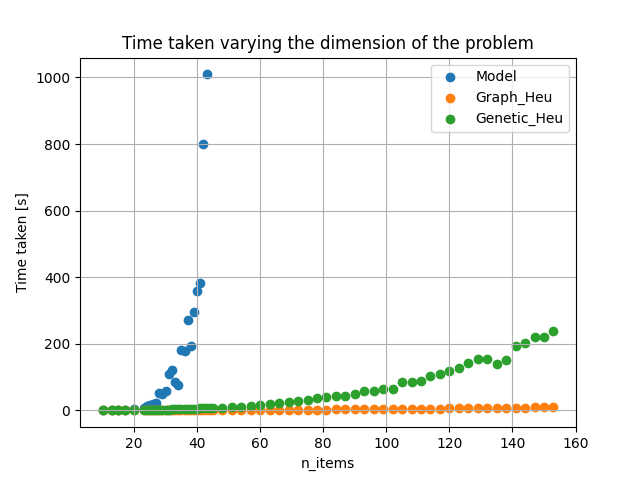
\includegraphics[width=0.66\textwidth]{times.png}}
\caption{Execution times of the model and the two heuristics}
\label{times}
\end{figure}

A few comments may be drawn from the image. First of all, as said in section 5, it is showed how, as the instances become bigger, the time needed by the model grows exponentially, and for more than 40-45 items a result cannot be produced in a reasonable time. Instead, the heuristics are able, even consistently increasing the instance size, to provide an output in a reduced amount of time. Genetic Heuristic starts struggling as $n_{items}$ passes 100, and it is in any case slower than Graph Heuristic, which indeed is very powerful, as even with very big instances it is able to run in just a bunch of seconds. The main reason behind this difference is in the architecture itself of the two algorithms. The more straightforward nature of Graph Heuristic (no need for stopping/convergence conditions) prevails over the great amount of (needed) overhead of Genetic Heuristic. The latter, moreover, is always iterated twice, as it tests two different initialization methods. 

\section{Conclusion}
In the end, it can be asserted that the described work has been able to perform an accurate analysis and modelling of the RKP problem and to develop useful heuristics for a fast solution of big instances. 
Graph Heuristic is the main result of this work and it performs nicely (as well as Genetic Heuristic) in terms of result, but always much better than the other in terms of execution time. 
The intention behind the construction of a second heuristic was in any case to offer a different perspective on the problem, as well as to determine a good alternative when the first heuristic (hardly ever) fails in determining an optimum.
Of course, the algorithms are not perfect, they occasionally fail and could certainly be improved: this might be indeed a possible extension of this work to be carried on in the future.

\printbibliography

\end{document}
